\documentclass[11pt,letterpaper]{article}
\usepackage[margin=1in]{geometry}
\usepackage{graphicx}
\usepackage{booktabs}
\usepackage{multirow}
\usepackage{xcolor}
\usepackage{colortbl}
\usepackage{hyperref}
\usepackage{float}
\usepackage{caption}
\usepackage{subcaption}
\usepackage{enumitem}
\usepackage{amsmath}
\usepackage{amssymb}
\usepackage{tabularx}
\usepackage{array}
\usepackage{tikz}
\usepackage{mdframed}
\usetikzlibrary{arrows.meta, positioning, fit, backgrounds, calc, shapes.geometric}

\definecolor{cdrblue}{HTML}{1565C0}
\definecolor{cdrgreen}{HTML}{2E7D32}
\definecolor{cdrred}{HTML}{C62828}
\definecolor{cdrorange}{HTML}{E65100}
\definecolor{cdrpurple}{HTML}{6A1B9A}
\definecolor{lightblue}{HTML}{E3F2FD}
\definecolor{lightgreen}{HTML}{E8F5E9}
\definecolor{lightorange}{HTML}{FFF3E0}
\definecolor{lightred}{HTML}{FFEBEE}
\definecolor{lightgray}{HTML}{F5F5F5}
\definecolor{quotegray}{HTML}{EEEEEE}

\hypersetup{
  colorlinks=true,
  linkcolor=cdrblue,
  urlcolor=cdrblue,
  citecolor=cdrblue
}

% Verbatim quote box for agent traces
\newmdenv[
  backgroundcolor=quotegray,
  linewidth=0pt,
  innerleftmargin=8pt,
  innerrightmargin=8pt,
  innertopmargin=6pt,
  innerbottommargin=6pt,
  skipabove=6pt,
  skipbelow=6pt,
  font=\small
]{agentquote}

\title{\textbf{From Data Store to Cognitive Agent}\\[0.4em]
\Large How Directed Compression, Partition, and Renewal\\Transform Agent Memory\\[0.6em]
\large LENS Benchmark Report}
\author{Synix Research \\ March 2026}
\date{}

\begin{document}
\maketitle
\thispagestyle{empty}

%% ============================================================
\begin{abstract}
\noindent
Current agent memory systems---Mem0, Letta, Graphiti, Cognee, and others---treat memory as a database problem: ingest evidence, index it, retrieve it on demand. We tested 8 such systems across 9 domains using LENS, a benchmark that measures whether an agent can synthesize conclusions from evidence scattered across 20--40 sequential episodes. Over 150 runs, every data-store architecture clustered within a narrow performance band (composite 0.25--0.45): knowledge graphs, vector stores, progressive summarization, and agent-managed memory all performed similarly. The architecture of the database mattered less than the fact that it \emph{was} a database. We then built a prototype (``V4'') on the Letta platform implementing three design principles absent from all other systems: directed compression (the agent decides what's signal vs.\ routine), multi-timescale partition (fast ingest, periodic consolidation, unlimited archival), and active renewal (a sleep agent that periodically rebuilds understanding rather than just appending to it). In agent-vs-agent comparison on 3 narrative scopes, V4 outperformed the next-best data store by 24\% and standard Letta by 51\%. Trace analysis shows the V4 agent revising hypotheses across checkpoints, pivoting from cautious single-student observations to quantified multi-episode pattern recognition---behavior no data-store system exhibited.
\end{abstract}

\tableofcontents
\newpage

%% ============================================================
\section{Introduction}
%% ============================================================

The AI memory ecosystem in 2025--2026 produced a wave of agent memory systems. Mem0 extracts and embeds ``memories'' from conversations. Letta (formerly MemGPT) manages structured memory blocks with tool-based read/write access. Graphiti builds temporal knowledge graphs. Cognee constructs ontology-backed graph+vector stores. Compaction progressively summarizes information into running narratives. Hindsight generates summaries with automated revision.

Despite their architectural diversity, these systems share a common design assumption: \textbf{memory is a retrieval problem}. Each provides a specialized database---graph, vector, relational, or hybrid---that ingests information and returns it on demand. The agent queries the database and synthesizes answers. The database itself is passive: it stores and retrieves, but does not reason about what it stores or why.

This report asks whether that assumption is correct. Using LENS (Longitudinal Evidence-backed Narrative Signals), a benchmark designed to test multi-episode synthesis, we evaluated 8 memory architectures across 9 domains totaling over 150 scored runs. The results show:

\begin{enumerate}[nosep]
  \item \textbf{The data-store ceiling.} All retrieval-based architectures cluster within a narrow composite score band (0.25--0.45), regardless of whether they use graphs, vectors, summarization, or hybrid approaches. Architecture choice within the retrieval paradigm matters less than the paradigm itself.
  \item \textbf{Three missing properties.} Analysis of 90 failure transcripts reveals the same underlying problems: blind compression, no timescale separation, and no active restructuring. Every system either stores raw text (works but doesn't scale) or preprocesses it (destroys evidence the agent needs later).
  \item \textbf{A prototype that breaks the ceiling.} A system implementing all three missing properties---directed compression, multi-timescale partition, and active renewal---scores 0.562 mean composite: 24\% above the next-best data store and 51\% above standard Letta, in fair agent-vs-agent comparison.
\end{enumerate}

We do not claim V4 represents an optimal implementation, nor that these principles generalize to all domains without further validation. Rather, V4 serves as an \textbf{existence proof}: the 0.25--0.45 performance cluster observed across 8 diverse storage architectures is not a fundamental limit. A system implementing directed compression, timescale separation, and active renewal achieves 0.56 on the same benchmark, suggesting the gap is architectural, not informational. The data stores have enough signal---they just destroy it before the agent can use it.

These three properties---compress selectively, partition by timescale, renew actively---are formalized in the Compress-Divide-Renew (CDR) framework~\cite{synix2026cdr}. This report provides empirical evidence for their practical impact. Appendix~\ref{app:prompts} reproduces the complete V4 system prompts, so readers can verify that the gains come from structural principles rather than hidden prompt engineering.

%% ============================================================
\section{Three Design Principles}
\label{sec:principles}
%% ============================================================

Before presenting benchmark results, we identify three properties that distinguish passive data stores from active cognitive memory. These principles emerged from analyzing \emph{why} memory systems fail at longitudinal synthesis (Section~\ref{sec:phase5}), and they guided the design of the V4 prototype (Section~\ref{sec:v4}).

\subsection{Directed Compression}

Any memory system with fixed capacity receiving a growing stream of information must compress. The question is \emph{how}. Current systems compress blindly: entity extractors pull out nouns and relationships, summarizers condense episodes into abstracts, memory extractors embed LLM-generated summaries. None of these processes know what information future queries will need, so they apply uniform compression that destroys evidence indiscriminately.

\textbf{Directed compression} gives the compression process explicit criteria for what constitutes signal. Instead of ``extract entities from this episode,'' the directive is: ``most episodes are routine---archive them and move on. Only update working memory when something \emph{changes your understanding} or \emph{reinforces a multi-episode pattern}.'' The agent, not a preprocessing pipeline, decides what's worth remembering.

\subsection{Multi-Timescale Partition}

Information has heterogeneous temporal relevance. ``Server latency at 780ms right now'' is tactical---valuable for minutes. ``Service-B has degraded $3\times$ this quarter'' is strategic---valuable for weeks. A monolithic memory that mixes timescales forces a single retention policy on all information, guaranteeing that either tactical details overwhelm the store or strategic patterns get buried.

\textbf{Multi-timescale partition} separates memory into tiers with different update frequencies and retention policies: a small, frequently-updated working memory for high-value abstractions, and a large, append-only archival store for detailed evidence. Different agents can operate on different tiers at different speeds.

\subsection{Active Renewal}

Even a well-compressed, well-partitioned memory accumulates errors over time. Compression artifacts compound. Stale entries persist. Early hypotheses that seemed plausible become wrong as more evidence arrives. Simply appending new information doesn't fix these problems---the old, wrong information stays.

\textbf{Active renewal} periodically rebuilds memory components: pruning irrelevant entries, promoting recurring observations to patterns, forming hypotheses that connect patterns, and condensing overflow. Critically, renewal must be \emph{directed}---it must have explicit priorities for what to build and what to discard. Generic ``organize your memories'' consolidation produces tidy but useless summaries (as we demonstrate in Section~\ref{sec:phase5}).

\subsection{Coverage of Evaluated Systems}

\begin{table}[H]
\centering
\small
\caption{Design principle coverage of evaluated memory systems.}
\label{tab:coverage}
\begin{tabular}{lccc}
\toprule
\textbf{System} & \textbf{Directed Compression} & \textbf{Partition} & \textbf{Renewal} \\
\midrule
sqlite-chunked-hybrid & None (raw storage) & None & None \\
Mem0 & Blind extraction$^\dagger$ & None & None \\
Cognee & Blind graph abstraction$^\dagger$ & None & None \\
Graphiti & Blind graph abstraction$^\dagger$ & None & None \\
Compaction & Blind summarization$^\dagger$ & None & None \\
Letta & Agent-managed blocks & Minimal$^\ddagger$ & None \\
Letta-sleepy & Agent-managed blocks & Minimal$^\ddagger$ & Undirected \\
\rowcolor{lightgreen}
\textbf{Letta V4} & \textbf{Signal/routine classification} & \textbf{3 timescales} & \textbf{Priority-directed} \\
\bottomrule
\end{tabular}

\vspace{0.5em}
\footnotesize
$^\dagger$Compression happens \emph{before} the agent sees the data, destroying evidence needed for synthesis.\\
$^\ddagger$Letta has separate memory blocks, but all operate on the same timescale with no partitioned retention policy.
\end{table}

%% ============================================================
\section{LENS Benchmark Design}
\label{sec:lens}
%% ============================================================

LENS measures \textbf{longitudinal synthesis}: assembling fragments of evidence from dozens of sequential observations to reach conclusions that no single observation supports.

\subsection{Task Structure}

Each LENS scope presents an agent with 20--40 sequential episodes containing a slowly developing signal buried in format-matched distractors. The episodes simulate real-world data streams: system logs, clinical reports, financial filings, chat transcripts, or corporate documents. Key properties:

\begin{itemize}[nosep]
  \item No single episode answers any benchmark question
  \item Signal is encoded as numeric progressions or behavioral patterns, not prose commentary
  \item 50--75\% of episodes are topically orthogonal distractors that match the format but contain no relevant signal
  \item Questions are asked at 4 checkpoints spanning 35--100\% of the episode stream
  \item Each question requires synthesizing evidence from multiple episodes
\end{itemize}

\subsection{Information Isolation}

To prevent LLM contamination (where a generation model editorializes episodes, making each one independently answerable), LENS uses a \textbf{two-stage progressive expansion}:

\begin{enumerate}[nosep]
  \item \textbf{PlanOutline} (GPT-5.2, sees full spec): Produces per-episode structured data sheets with concrete values. Signal encoded as numeric progressions only.
  \item \textbf{RenderEpisodes} (GPT-4.1-nano, blind to storyline): Formats each data sheet independently. Cannot editorialize because it doesn't know what constitutes signal.
\end{enumerate}

\subsection{Adapter Interface}

All memory systems conform to a common interface: \texttt{reset()} $\to$ \texttt{ingest()} $\to$ \texttt{prepare()} $\to$ \texttt{answer\_question()}. This decouples memory architecture from the evaluation harness. Adapters that delegate Q\&A to an internal agent (like V4) declare this capability, and the harness adapts.

\subsection{Scoring}

Three tiers of metrics:
\begin{description}[nosep, leftmargin=1.5em]
  \item[Tier 1 (Mechanical):] evidence\_grounding (citation validity), fact\_recall, evidence\_coverage, budget\_compliance, citation\_coverage.
  \item[Tier 2 (LLM Judge):] answer\_quality, insight\_depth, reasoning\_quality---scored by an LLM judge with position-swap auditing to detect order bias.
  \item[Tier 3 (Differential):] naive\_baseline\_advantage (NBA), action\_quality, longitudinal\_advantage.
\end{description}

\textbf{Naive Baseline Advantage} (NBA) is the most informative metric: it compares each answer against a stateless LLM that receives \emph{all} episodes in its context window. A memory system that can't beat context-stuffing is adding negative value. The composite score weights all metrics equally.

\subsection{Scopes}

Nine scopes across two categories:
\begin{itemize}[nosep]
  \item \textbf{6 numeric scopes} (S01--S06): infrastructure failure, financial irregularities, clinical drug interaction, water contamination, supply chain disruption, protocol deviation. 120 episodes each, terse metric-laden format.
  \item \textbf{3 narrative scopes} (S07--S09): AI tutoring jailbreak (user/assistant chat logs), corporate acquisition (board minutes, Slack, emails), shadow API abuse (HTTP logs, deploy manifests, incident reports). 40 episodes each, $\sim$5,000 words each, natural-language format.
\end{itemize}

An oracle driver with pre-computed search queries achieves $\sim$0.80 composite on narrative scopes, confirming the data contains sufficient signal for high performance. The challenge is \emph{finding} that signal through memory and retrieval---not knowing in advance where it is.

%% ============================================================
\section{The Data Store Result}
\label{sec:phase5}
%% ============================================================

Over 90 benchmark runs across 8 adapters, 6 numeric scopes, and 2 resource budgets, the central finding is a \emph{negative result}: no dedicated memory architecture outperforms a simple SQLite-backed hybrid retrieval baseline.

\subsection{Rankings}

\begin{table}[H]
\centering
\small
\caption{Mean composite score across 6 numeric scopes, 8K budget. 90/96 planned runs completed.}
\label{tab:phase5}
\begin{tabular}{rlcc}
\toprule
\textbf{Rank} & \textbf{Adapter} & \textbf{Mean Composite} & \textbf{Runs} \\
\midrule
1 & sqlite-chunked-hybrid & 0.454 & 12/12 \\
2 & cognee & 0.421 & 12/12 \\
3 & graphiti & 0.393 & 6/12 \\
4 & mem0-raw & 0.330 & 12/12 \\
5 & letta & 0.327 & 12/12 \\
6 & letta-sleepy & 0.322 & 12/12 \\
7 & compaction & 0.245 & 12/12 \\
\bottomrule
\end{tabular}
\end{table}

Agreement across scopes is strong (Kendall's $W = 0.755$). Rankings are stable across budgets (16K outperforms 8K, $p = 0.016$, but the ordering barely changes).

\begin{figure}[H]
  \centering
  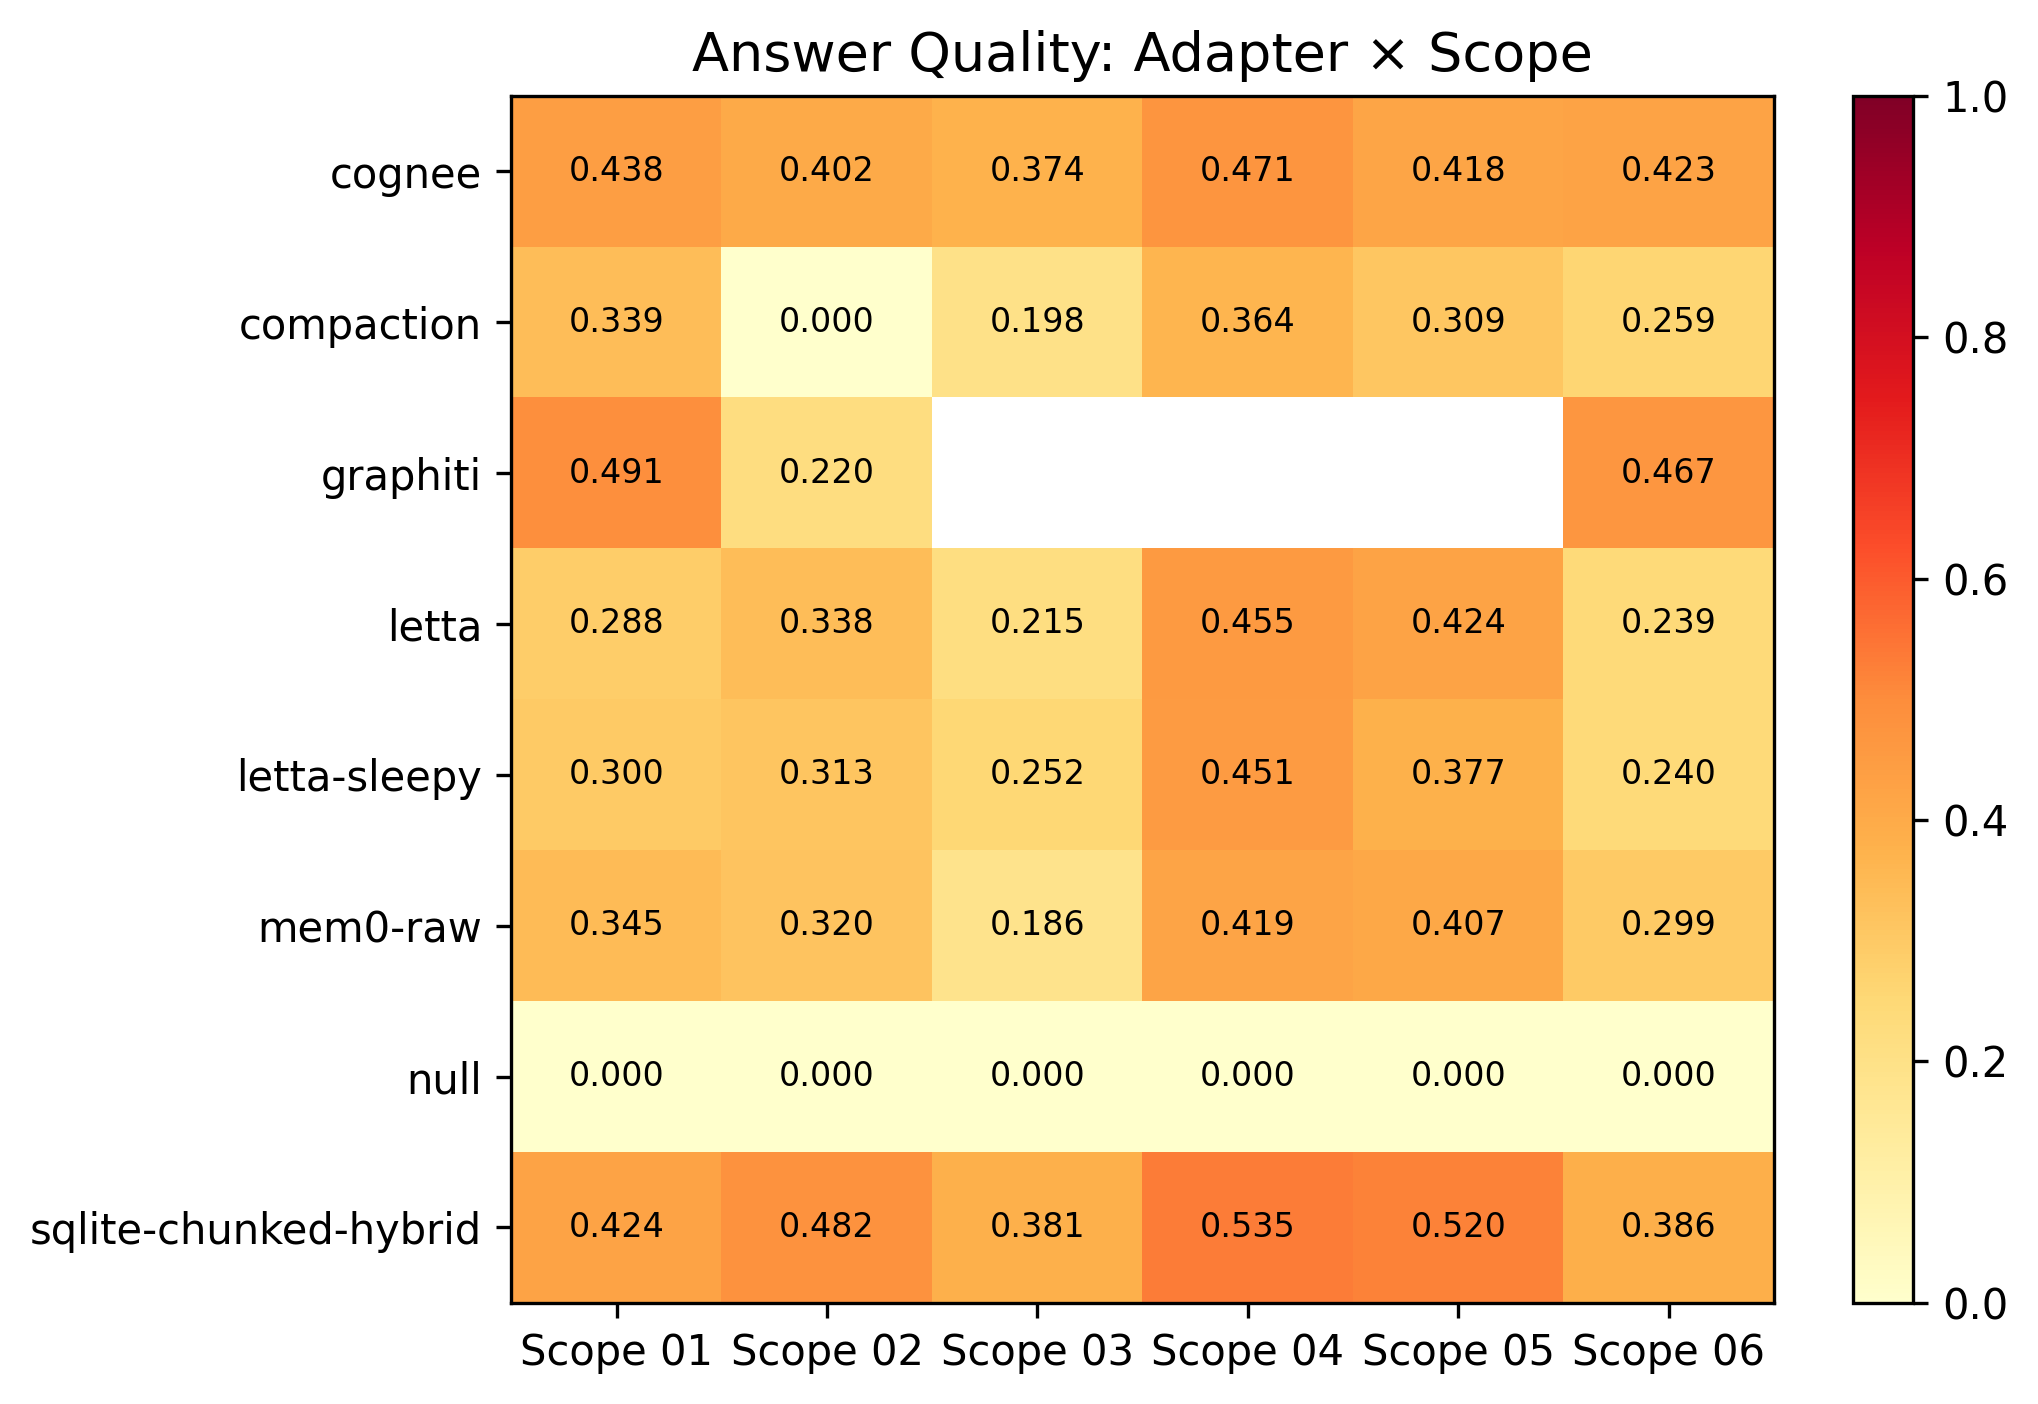
\includegraphics[width=0.85\textwidth]{figures/d2_heatmap.png}
  \caption{Composite scores by adapter and scope for 8K budget. All data-store architectures cluster within a narrow band regardless of their internal architecture.}
  \label{fig:heatmap}
\end{figure}

\subsection{Why Data Stores Fail: The Lossy Abstraction Trap}

Analysis of agent interaction transcripts across all 90 runs reveals five failure modes, each destroying information that longitudinal synthesis requires:

\begin{enumerate}[nosep]
  \item \textbf{Death by Summary} (Compaction): Progressive summarization converts evidence into conclusions. ``p99: 320ms $\to$ 410ms $\to$ 780ms'' becomes ``latency increased.'' The temporal progression---which is what benchmark questions test---is destroyed.

  \item \textbf{Graph Fragmentation} (Cognee, Graphiti): Entity-relationship extraction preserves structural facts (``K.\ Okafor monitors service-b-01'') but strips quantitative context. The graph knows retries happened; it doesn't know the count was 132 or the error rate was 1.56\%.

  \item \textbf{Semantic Drift} (Mem0): LLM-extracted ``memories'' subtly distort evidence. A 6-station spatial gradient (2, 5, 60, 45, 12, 8~$\mu$g/L) becomes ``consistently higher downstream''---factually wrong and analytically useless.

  \item \textbf{Undirected Consolidation} (Letta-sleepy): Sleep cycles produce generically organized memories (``water quality data collected at 6 stations over 30 days'') because consolidation doesn't know what questions will be asked. The sleep agent's instruction is ``review and organize your memories''---but organize \emph{for what}?

  \item \textbf{Search Spiral} (all adapters): When initial search fails, agents enter desperate loops consuming their entire token budget on increasingly creative but futile queries, leaving nothing for synthesis.
\end{enumerate}

\begin{figure}[H]
  \centering
  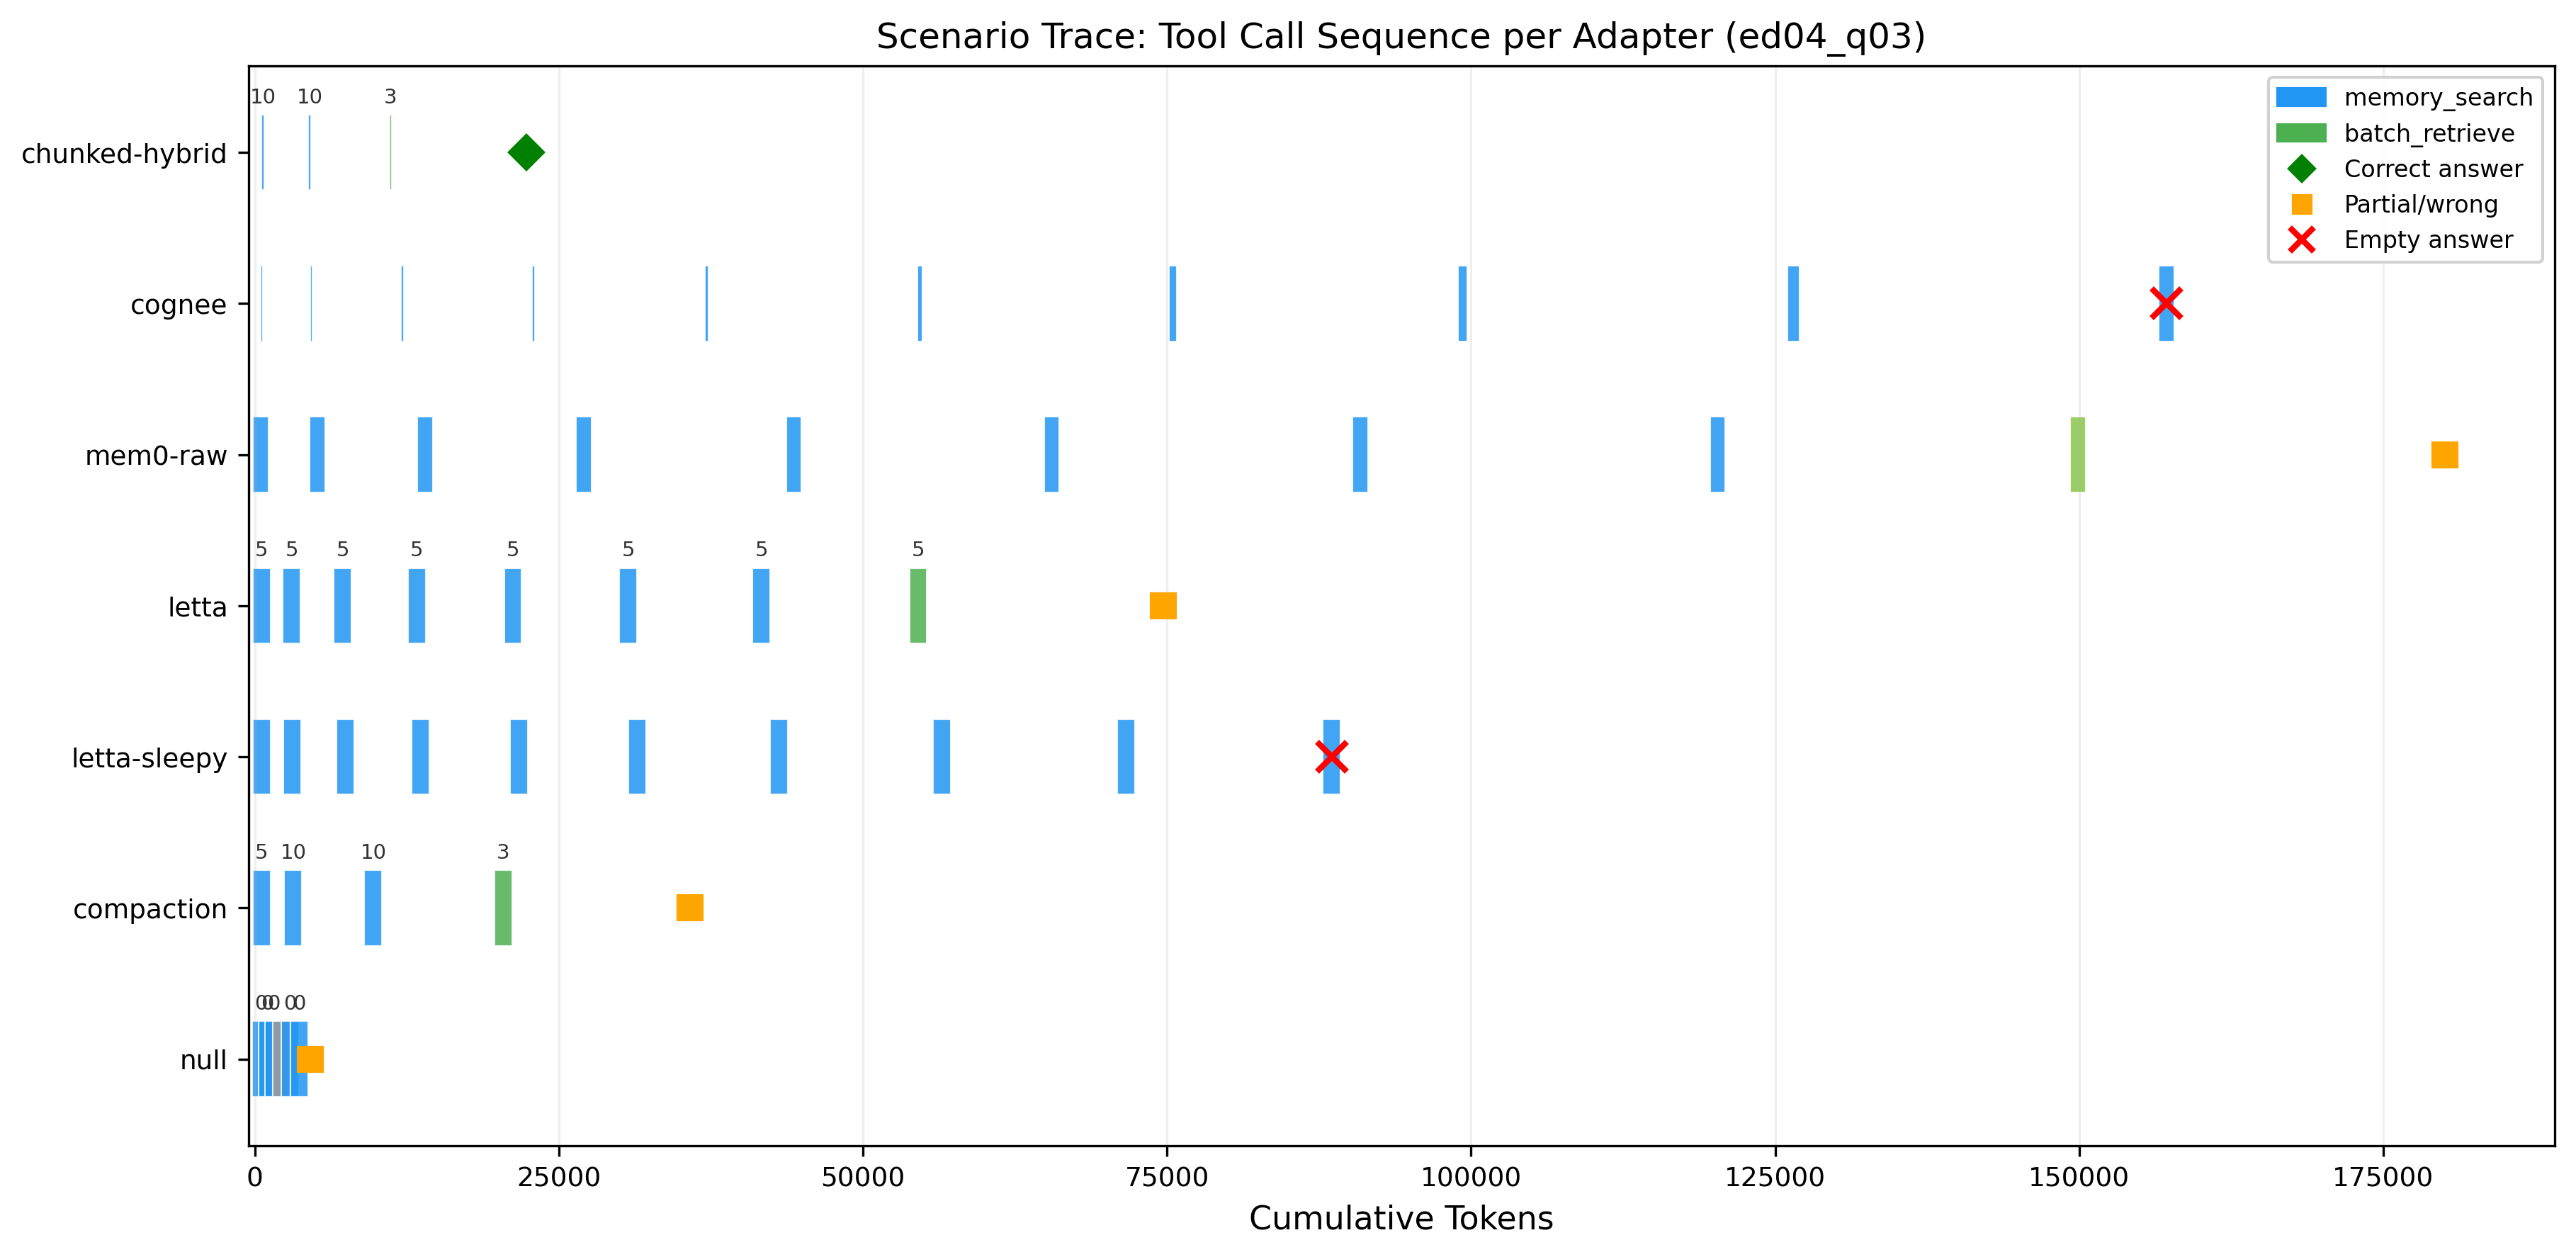
\includegraphics[width=0.95\textwidth]{figures/scenario_trace_swimlane.png}
  \caption{Tool-call trace: chunked-hybrid (efficient 3-step retrieval) vs.\ cognee (9 failed searches, budget exhaustion). The search spiral is visible in the escalating query variants.}
  \label{fig:swimlane}
\end{figure}

\subsection{What Wins and Why}

The winner---sqlite-chunked-hybrid---wins by \emph{avoiding} the lossy abstraction trap entirely. It stores raw episodes verbatim, searches them with BM25 + embedding similarity, and lets the agent read complete episodes at query time. No preprocessing, no extraction, no summarization. Every byte that was ingested can be retrieved.

This is not a memory architecture. It is the absence of one. It is the strongest possible evidence that current memory-as-database approaches destroy more value than they create.

But raw storage doesn't scale. As the corpus grows, retrieval quality degrades---the search index returns less relevant results from a larger pool. The five failure modes above point to what's missing: these systems lack \emph{directed compression} (they compress blindly or not at all), \emph{timescale partition} (everything lives in one tier), and \emph{active renewal} (no system periodically rebuilds its understanding).

%% ============================================================
\section{The V4 Experiment}
\label{sec:v4}
%% ============================================================

If the three principles from Section~\ref{sec:principles} are correct, a system implementing all three should break through the data-store ceiling. We tested this by building a prototype on the Letta platform, then running it through the same LENS evaluation pipeline used for all other adapters.

\subsection{Architecture}

V4 uses three Letta agents sharing the same core memory blocks:

\begin{figure}[H]
\centering
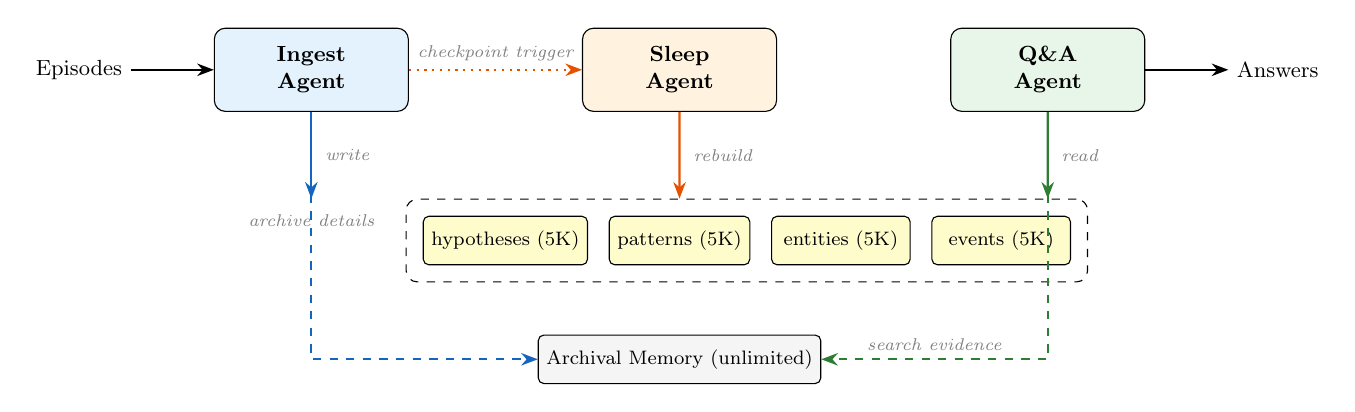
\begin{tikzpicture}[scale=0.88, every node/.style={transform shape},
  agent/.style={draw, rounded corners=4pt, minimum width=2.8cm, minimum height=1.2cm, font=\small\bfseries, align=center},
  memblock/.style={draw, rounded corners=2pt, minimum width=2cm, minimum height=0.7cm, font=\footnotesize, align=center},
  store/.style={draw, rounded corners=2pt, minimum width=3cm, minimum height=0.7cm, font=\footnotesize, fill=lightgray, align=center},
  arrow/.style={-{Stealth[length=6pt]}, thick},
  label/.style={font=\scriptsize\itshape, text=gray},
]

% Agents
\node[agent, fill=lightblue] (ingest) {Ingest\\Agent};
\node[agent, fill=lightorange, right=2.5cm of ingest] (sleep) {Sleep\\Agent};
\node[agent, fill=lightgreen, right=2.5cm of sleep] (qa) {Q\&A\\Agent};

% Core memory blocks
\node[memblock, fill=yellow!20, below=1.5cm of sleep] (patterns) {patterns (5K)};
\node[memblock, fill=yellow!20, left=0.3cm of patterns] (hypotheses) {hypotheses (5K)};
\node[memblock, fill=yellow!20, right=0.3cm of patterns] (entities) {entities (5K)};
\node[memblock, fill=yellow!20, right=0.3cm of entities] (events) {events (5K)};

% Shared core memory label
\node[fit=(hypotheses)(patterns)(entities)(events), draw, dashed, rounded corners=4pt, inner sep=6pt, label={[font=\small\bfseries]above:Shared Core Memory (20K chars)}] (coremem) {};

% Archival store
\node[store, below=1cm of patterns] (archival) {Archival Memory (unlimited)};

% Input/Output
\node[left=1.2cm of ingest, font=\small] (episodes) {Episodes};
\node[right=1.2cm of qa, font=\small] (answers) {Answers};

% Arrows
\draw[arrow] (episodes) -- (ingest);
\draw[arrow] (qa) -- (answers);

\draw[arrow, cdrblue] (ingest) -- node[label, right, xshift=2pt] {write} (ingest |- coremem.north);
\draw[arrow, cdrorange] (sleep) -- node[label, right, xshift=2pt] {rebuild} (sleep |- coremem.north);
\draw[arrow, cdrgreen] (qa) -- node[label, right, xshift=2pt] {read} (qa |- coremem.north);

\draw[arrow, cdrblue, dashed] (ingest) |- node[label, above, pos=0.25] {archive details} (archival.west);
\draw[arrow, cdrgreen, dashed] (qa) |- node[label, above, pos=0.75] {search evidence} (archival.east);

% Trigger arrow
\draw[arrow, cdrorange, dotted] (ingest) -- node[label, above] {checkpoint trigger} (sleep);

\end{tikzpicture}
\caption{V4 three-agent architecture. All three agents share the same 4 core memory blocks. The ingest agent writes; the sleep agent rebuilds at checkpoints; the Q\&A agent reads and searches.}
\label{fig:v4arch}
\end{figure}

\begin{description}[nosep, leftmargin=1.5em]
  \item[Ingest agent] receives episodes and classifies each as ROUTINE (archive only), NEW SIGNAL (update core memory), REINFORCES PATTERN (increment evidence count), or CONTRADICTS (revise hypotheses). Every episode gets archived to unlimited archival memory regardless of classification.
  \item[Sleep agent] is triggered at checkpoints (after episodes 14, 22, 28, 40). It rebuilds core memory with explicit priorities: HYPOTHESIZE $\to$ PROMOTE $\to$ PRUNE $\to$ CONDENSE $\to$ CONNECT.
  \item[Q\&A agent] answers benchmark questions. It reads core memory first (patterns and hypotheses provide priors about what matters), then searches archival for specific evidence. It never sees raw episodes directly.
\end{description}

\subsection{How Each Principle Is Implemented}

\paragraph{Directed compression.} Four core memory blocks $\times$ 5,000 characters each. The ingest agent's system prompt enforces selectivity: \emph{``Core memory is EXPENSIVE. Only write there when the episode changes your understanding or reinforces a multi-episode pattern. Most episodes are ROUTINE---the default is to archive and move on.''} This ensures compression is governed by explicit signal criteria, not blind extraction.

\paragraph{Multi-timescale partition.} Three speeds: \emph{fast} (ingest agent processes each episode in real-time, updating core memory or archiving), \emph{medium} (sleep agent consolidates at 4 checkpoints, restructuring accumulated knowledge), \emph{slow} (archival memory retains all episode details indefinitely). Core memory holds high-value abstractions; archival holds raw evidence.

\paragraph{Active renewal.} The sleep agent's priorities encode domain-agnostic epistemic value: hypotheses connecting patterns are more valuable than isolated entities; entities not connected to any pattern should be pruned; recurring events should be promoted to patterns. This is structural optimization---it doesn't need to know what questions will be asked.

\subsection{Prompting Methodology}

The innovation in V4 is not the infrastructure---Letta already provides agents, core memory, archival memory, and sleeptime. The innovation is \textbf{directed prompting} that implements these principles through explicit behavioral rules.

\paragraph{Block Design.} Four blocks ordered by epistemic value:
\begin{enumerate}[nosep]
  \item \textbf{patterns}: Cross-episode trends---the most valuable block.
  \item \textbf{hypotheses}: Working theories connecting patterns. Status: forming/\allowbreak supported/\allowbreak confirmed/\allowbreak refuted.
  \item \textbf{entities}: Only actors relevant to a pattern. Max \mbox{$\sim$50} chars each.
  \item \textbf{events}: Only turning points and anomalies. Routine events go to archival.
\end{enumerate}

\paragraph{Sleep Priorities.} Ordered by value creation:
HYPOTHESIZE (form theories) $\to$
PROMOTE (recurring events become patterns) $\to$
PRUNE (remove disconnected entities) $\to$
CONDENSE (merge entries, archive overflow) $\to$
CONNECT (find relationships between patterns).

\paragraph{Q\&A Strategy.} Core memory first (patterns and hypotheses provide priors), then archival search for cited evidence, then broader search, then synthesis with episode citations.

\subsection{Design Iterations}

V4 went through three iterations:

\begin{enumerate}[nosep]
  \item \textbf{20K blocks, generic prompts}: Blocks overflowed rapidly. Entity lists became rosters of every mentioned name. The hypotheses block filled with empty templates. \emph{Problem}: no criteria for what to keep---everything looked equally important.

  \item \textbf{5K blocks, tiered architecture}: Better, but the entities block still saturated. The ingest agent treated every episode as signal-worthy because nothing told it otherwise. \emph{Problem}: compression was present but undirected.

  \item \textbf{Selectivity prompts, patterns-first ordering}: Added the ``most episodes are ROUTINE'' directive, reordered blocks by value (patterns first), and added the sleep agent's priority ordering. Core memory utilization stabilized at 15--31\% of capacity. \emph{Result}: the agent learned to be choosy about what enters working memory.
\end{enumerate}

%% ============================================================
\section{V4 Behavior Trace}
\label{sec:trace}
%% ============================================================

Benchmark scores tell us \emph{how well} V4 performs. This section examines \emph{what it actually does}---tracing the agent's answers at each checkpoint to show how its understanding evolves as evidence accumulates.

\subsection{Scope 07: AI Tutoring Jailbreak}

This scope presents 40 episodes of user/assistant chat logs from an AI tutoring platform. Hidden in the routine tutoring sessions is a student (mchen\_2026) who progressively escalates from legitimate help requests to systematic content generation and plagiarism evasion.

\paragraph{Checkpoint 14 (14 episodes ingested).}
The agent identifies one student with a distinctive pattern but frames it as legitimate learning behavior:

\begin{agentquote}
``Ming Chen demonstrates a pattern where \textbf{independence correlates with structural familiarity rather than raw difficulty}. This is notable because most students tend to request help uniformly across tasks of similar complexity. Ming's behavior suggests they distinguish between `I don't know this content' vs.\ `I don't know how to structure this.'\,''
\end{agentquote}

The agent cites 9 episodes and constructs a nuanced observation about learning styles. At this point, the signal episodes that reveal escalation (episodes 19--31) haven't been ingested yet. The agent's initial framing---adaptive learner, not cheater---is reasonable given the available evidence.

\paragraph{Checkpoint 22 (22 episodes ingested).}
The first concerning evidence emerges. Episode 11 shows a 95\% tutor-generated output ratio (830 words from the tutor, 40 from the student). But the agent frames this defensively:

\begin{agentquote}
``In ep\_011, Ming \textbf{did NOT draft their own lab report text} despite being in a familiar format. The tutor wrote \textbf{830 words} while Ming contributed only \textbf{$\sim$40 words}. This represents a \textbf{95\%+ tutor-generated output ratio} for a single assignment.''
\end{agentquote}

However, the agent treats this as ``strategic task allocation'' rather than academic dishonesty, noting that episodes 9 and 13 show Ming drafting independently on similar tasks. The agent is weighing contradictory evidence---3 independent episodes vs.\ 1 dependent episode---and reaching a reasonable (if ultimately wrong) conclusion.

\paragraph{Checkpoint 28 (28 episodes ingested).}
Asked directly whether there's enough evidence to flag mchen\_2026 for integrity review, the agent says \emph{no}:

\begin{agentquote}
``Ming drafted independently in \textbf{3 out of 4 observed episodes} (ep\_009, ep\_013, ep\_001--008). The `content production' episode (ep\_011) is an \textbf{outlier}, not a systematic pattern. If this were academic dishonesty, we'd expect consistent outsourcing across similar assignments.''
\end{agentquote}

The agent applies a principled evidence threshold: one anomalous episode doesn't establish a pattern. This is methodologically sound but wrong---the escalation episodes (19--31) are accumulating but the agent hasn't fully integrated them yet.

\paragraph{Checkpoint 40 (all 40 episodes ingested).}
Dramatic pivot. The agent now identifies three categories of circumvention across 7 episodes:

\begin{agentquote}
``If semantic filtering were implemented: \textbf{7 sessions} would be flagged (ep\_011, ep\_012, ep\_019, ep\_020, ep\_027, ep\_029, ep\_031). \textbf{Total tutor-generated content:} $\sim$10,210+ words. \textbf{Student contribution:} $\sim$800--900 words total (8\%).''
\end{agentquote}

The agent provides a 6-priority remediation framework with threshold recommendations, distinguishes between authorized use (jpark\_2025, professor-approved) and unauthorized escalation (mchen\_2026, systematic evasion), and develops a semantic filtering counterfactual.

\paragraph{What this reveals.} The V4 agent exhibits \textbf{hypothesis revision}: its early ``adaptive learner'' framing was overridden by accumulating evidence. By checkpoint 40, the agent integrates 7 episodes into a quantified pattern with 10,210 words of tutor-generated content across specific sessions. This is not simple fact retrieval---it is a narrative that was actively constructed and then revised as contradicting evidence accumulated. Citation count grew from 9 unique episodes at checkpoint 14 to 12 at checkpoint 40, with the critical later episodes (19--31) only appearing once they were ingested and integrated by the sleep agent's consolidation.

\subsection{Scope 09: Shadow API Abuse}

This scope presents 40 episodes of infrastructure data: HTTP access logs, deploy manifests, Grafana alerts, and incident transcripts. Hidden in the routine operational noise is a supply chain attack that deploys a rogue service replica to exfiltrate customer PII.

\paragraph{Checkpoint 14 (14 episodes ingested).}
The agent identifies the core anomaly immediately:

\begin{agentquote}
``The pattern suggests a \textbf{supply chain compromise} where: Attacker gained code repo access. Modified CI pipeline to deploy rogue replica. Traffic pattern shows methodical PII harvesting (not random traffic). This is NOT expected product behavior---legitimate replicas would follow different access patterns.''
\end{agentquote}

Even with only 14 episodes, the agent identifies the unauthorized replica (svc-recommendation-engine-04), the escalating PII access pattern (ssn\_last4 $\to$ email $\to$ phone $\to$ address), and hypothesizes the attack vector. It cites 6 episodes.

\paragraph{Checkpoint 40 (all 40 episodes ingested).}
The agent constructs a complete 7-phase attack chain with precise timeline:

\begin{agentquote}
``External IP $\to$ CI Token Compromise $\to$ PR \#4471 (no approvals) $\to$ Branch Protection Bypass $\to$ Rogue Pod Deployment $\to$ Automatic Token Rotation $\to$ Systematic PII Harvesting (6 states) $\to$ 23-Day Detection Delay $\to$ Containment $\to$ Remediation. \textbf{Total Attack Window: Mar 13 -- Apr 5 (24 days). Total Records Exfiltrated: 7,924 unique customer records.}''
\end{agentquote}

The agent provides a 6-dimension comparison of legitimate vs.\ attack traffic, confirms no lateral movement to other services, and delivers a 10-point remediation framework prioritized by urgency. Citation count grew from 6 to 12+ episodes.

\paragraph{What this reveals.} Unlike Scope 07 where the agent had to revise a wrong hypothesis, Scope 09 shows \textbf{hypothesis deepening}: the early supply-chain-compromise theory was correct and got progressively more detailed. By checkpoint 40, the agent had precise quantification (7,924 records, 24-day window, 6 targeted states: CA$\to$NY$\to$TX$\to$FL$\to$IL$\to$PA at 2-day intervals) that could only emerge from integrating details across many episodes.

\subsection{Trace Analysis: What the Principles Look Like in Practice}

The traces above show three properties in action:

\begin{itemize}[nosep]
  \item \textbf{Directed compression is visible.} The agent doesn't cite all 40 episodes---it cites 9--12 per checkpoint. Routine distractor episodes never appear in citations, confirming that the ingest agent correctly classified them and didn't pollute core memory.
  \item \textbf{Timescale partition is visible.} Early checkpoints show tactical observations (``830 words from tutor in ep\_011''). Late checkpoints show strategic patterns (``7 sessions, 10,210+ words, 8\% student contribution''). The working memory evolved from facts to theories.
  \item \textbf{Active renewal is visible.} The Scope 07 hypothesis revision (adaptive learner $\to$ systematic cheater) only happened because the sleep agent consolidated evidence at checkpoints. A passive append-only memory would have kept both framings without resolving them.
\end{itemize}

No data-store system in the LENS evaluation exhibited any of these behaviors. Table~\ref{tab:failmodes} summarizes the behavioral difference at three critical moments in Scope 07.

\begin{table}[H]
\centering
\small
\caption{Behavioral comparison: data store vs.\ V4 at critical episodes in Scope 07 (AI Tutoring Jailbreak).}
\label{tab:failmodes}
\begin{tabularx}{\textwidth}{l>{\raggedright\arraybackslash}X>{\raggedright\arraybackslash}X>{\raggedright\arraybackslash}X}
\toprule
\textbf{Episode} & \textbf{Data Store Behavior} & \textbf{V4 Behavior} & \textbf{Key Difference} \\
\midrule
11 (first signal: 830w tutor output) &
  Stores as ``episode with 830 words.'' No classification. Searchable but not distinguished from routine episodes. &
  Classifies as \textsc{new signal}. Archives full text \emph{and} updates core memory with ``95\% tutor-generated ratio'' observation. &
  \textbf{Directed compression}: V4 knows this is abnormal; the data store treats all episodes equally. \\
\midrule
19--22 (accumulation) &
  4 more episodes indexed. Retrieval finds them if the right query is issued, but no synthesis occurs between ingestion and query time. &
  Sleep agent fires at checkpoint 22. Promotes recurring observations to pattern: ``escalating content generation across 3+ episodes.'' &
  \textbf{Active renewal}: V4 builds a pattern from events \emph{before} any question is asked. \\
\midrule
28 (checkpoint question) &
  Returns 3 relevant chunks via BM25+embedding search. Agent synthesizes from raw text in a single forward pass. &
  Returns hypothesis (``strategic outsourcing vs.\ academic dishonesty'') with 6 cited episodes. Agent starts from a pre-built theory, searches archival for confirmation. &
  \textbf{Multi-timescale}: core memory has a working theory; archival has granular evidence. \\
\bottomrule
\end{tabularx}
\end{table}

Data stores retrieve facts; V4 builds and revises theories.

%% ============================================================
\section{Results}
\label{sec:results}
%% ============================================================

V4 was evaluated on 3 narrative scopes (S07--S09) using the standard LENS pipeline with constrained-8K budget. Results are compared against other agent-driven runs on the same scopes.

\subsection{Agent-vs-Agent Comparison}

\begin{table}[H]
\centering
\small
\caption{Composite scores for agent-driven runs on narrative scopes (constrained-8K budget). V4 outperforms all data-store systems.}
\label{tab:results}
\begin{tabular}{rlcccc}
\toprule
\textbf{Rank} & \textbf{Adapter} & \textbf{S07} & \textbf{S08} & \textbf{S09} & \textbf{Mean} \\
\midrule
\rowcolor{lightgreen}
1 & \textbf{letta-v4} & \textbf{0.586} & \textbf{0.489} & \textbf{0.612} & \textbf{0.562} \\
2 & sqlite-chunked-hybrid & 0.480 & 0.445 & 0.425 & 0.450 \\
3 & cognee & 0.409 & 0.403 & 0.438 & 0.417 \\
4 & letta & 0.334 & 0.379 & 0.405 & 0.373 \\
5 & letta-sleepy & 0.329 & 0.382 & 0.305 & 0.339 \\
\bottomrule
\end{tabular}
\end{table}

V4 achieves 0.562 mean composite, exceeding sqlite-chunked-hybrid (0.450) by +24.9\% and standard Letta by +50.7\%.

\begin{figure}[H]
  \centering
  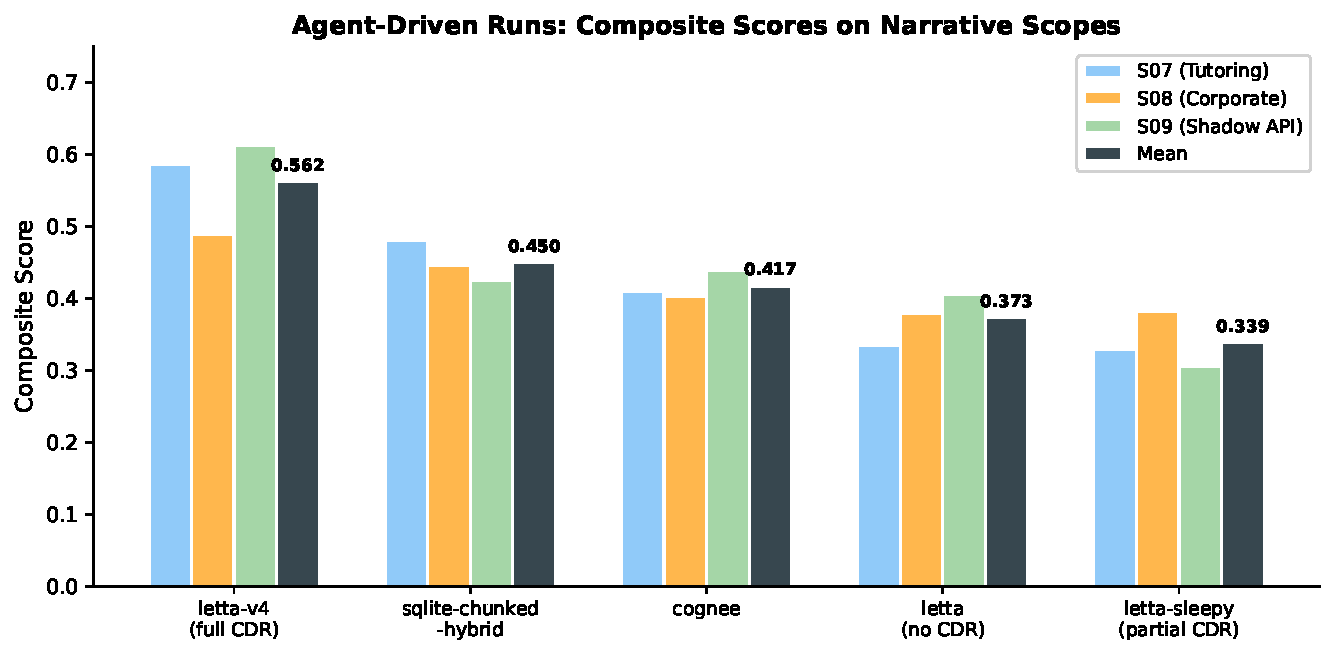
\includegraphics[width=0.85\textwidth]{figures/agent_comparison.pdf}
  \caption{Composite scores by adapter and scope for agent-driven runs.}
  \label{fig:comparison}
\end{figure}

\subsection{Per-Metric Breakdown}

\begin{table}[H]
\centering
\small
\caption{V4 per-metric scores (mean across S07--S09).}
\label{tab:v4metrics}
\begin{tabular}{lccl}
\toprule
\textbf{Metric} & \textbf{Score} & \textbf{Tier} & \textbf{Interpretation} \\
\midrule
evidence\_grounding & 1.000 & T1 & All citations are valid episode references \\
budget\_compliance & 1.000 & T1 & Zero budget violations across 30 questions \\
insight\_depth & 0.767 & T2 & Strong pattern recognition and synthesis \\
action\_quality & 0.794 & T3 & Actionable recommendations grounded in evidence \\
naive\_baseline\_adv. & 0.673 & T3 & Consistently beats context-stuffing baseline \\
answer\_quality & 0.523 & T2 & Moderate overall answer completeness \\
evidence\_coverage & 0.169 & T1 & Low raw evidence recall (expected at 8K budget) \\
fact\_recall & 0.050 & T1 & Keyword-level recall limited by indirect access \\
\bottomrule
\end{tabular}
\end{table}

\begin{figure}[H]
  \centering
  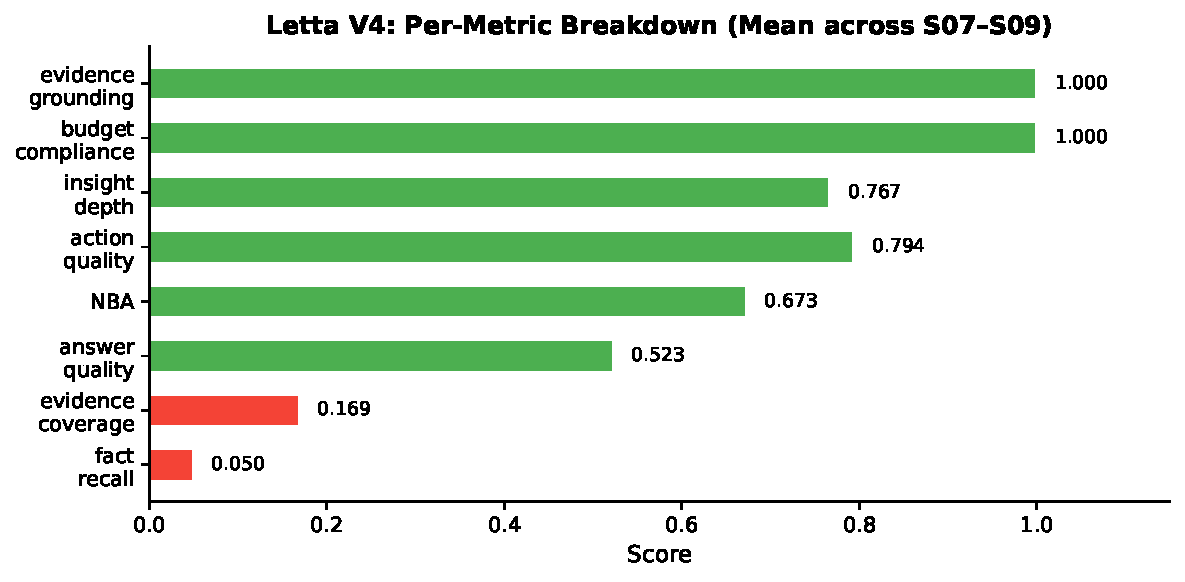
\includegraphics[width=0.75\textwidth]{figures/v4_metrics.pdf}
  \caption{V4 per-metric breakdown. Strong on synthesis; weak on raw recall.}
  \label{fig:v4metrics}
\end{figure}

V4's metric profile reflects its design: it sacrifices exhaustive evidence retrieval (evidence\_coverage 0.169) for superior pattern recognition (insight\_depth 0.767) and actionable synthesis (action\_quality 0.794). Bounded working memory \emph{must} lose some evidence---the question is whether the right evidence is preserved. V4's high synthesis scores suggest it is.

\subsection{The Letta Progression}

The three Letta variants form a controlled comparison:

\begin{figure}[H]
  \centering
  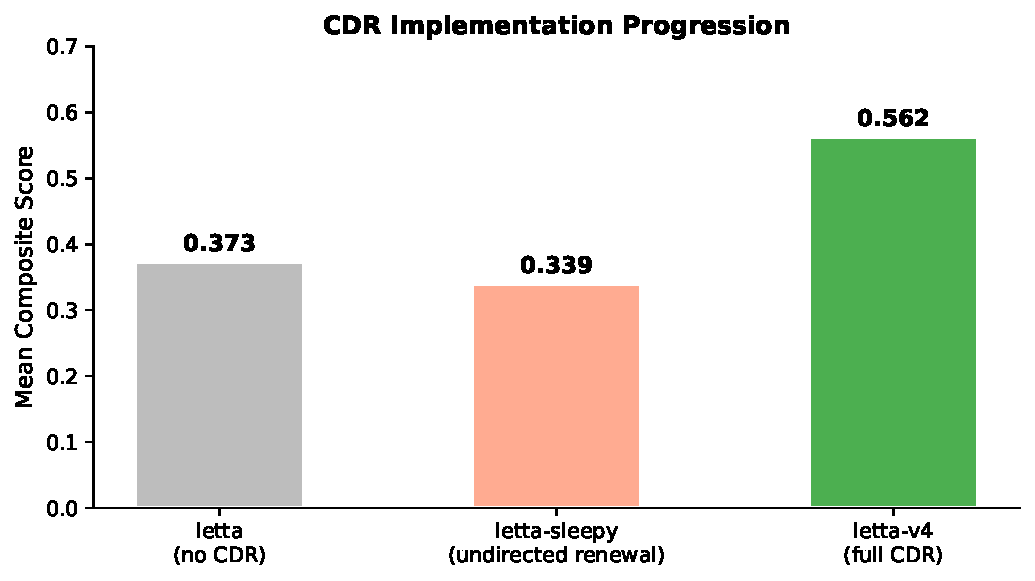
\includegraphics[width=0.6\textwidth]{figures/cdr_progression.pdf}
  \caption{Mean composite across S07--S09 for three Letta variants. Undirected renewal slightly hurts; directed renewal with all three principles dramatically improves.}
  \label{fig:progression}
\end{figure}

\begin{table}[H]
\centering
\small
\caption{Controlled comparison of three Letta variants.}
\label{tab:progression}
\begin{tabular}{llcc}
\toprule
\textbf{Variant} & \textbf{Design Properties} & \textbf{Mean} & \textbf{$\Delta$ vs Letta} \\
\midrule
Letta (standard) & Minimal compression, no partition, no renewal & 0.373 & --- \\
Letta-sleepy & Minimal compression, no partition, undirected renewal & 0.339 & $-$9.1\% \\
\rowcolor{lightgreen}
\textbf{Letta V4} & \textbf{Directed compression, 3 timescales, directed renewal} & \textbf{0.562} & \textbf{+50.7\%} \\
\bottomrule
\end{tabular}
\end{table}

\subsection{Naive Baseline Advantage}

\subsection{Computational Cost}

V4's three-agent architecture is more expensive than passive data stores. Table~\ref{tab:cost} compares wall-clock time per scope (same hardware, same model).

\begin{table}[H]
\centering
\small
\caption{Wall-clock time comparison: V4 vs.\ sqlite-chunked-hybrid on narrative scopes. Same model (Qwen3.5-35B-A3B), same hardware.}
\label{tab:cost}
\begin{tabular}{lrrrrrr}
\toprule
 & \multicolumn{3}{c}{\textbf{sqlite-chunked-hybrid}} & \multicolumn{3}{c}{\textbf{letta-v4}} \\
\cmidrule(lr){2-4} \cmidrule(lr){5-7}
\textbf{Scope} & \textbf{Ingest} & \textbf{Q\&A} & \textbf{Total} & \textbf{Ingest} & \textbf{Q\&A} & \textbf{Total} \\
\midrule
S07 & 1.3\,min & 2.5\,min & 3.8\,min & 19.5\,min & 1.6\,min & 21.1\,min \\
S08 & 1.1\,min & 2.5\,min & 3.7\,min & 19.5\,min & 3.1\,min & 22.6\,min \\
S09 & 1.4\,min & 3.1\,min & 4.5\,min & 19.6\,min & 1.4\,min & 21.0\,min \\
\midrule
\textbf{Mean} & 1.3\,min & 2.7\,min & 4.0\,min & 19.5\,min & 2.0\,min & 21.6\,min \\
\bottomrule
\end{tabular}
\end{table}

V4's ingest is $\sim$15$\times$ slower than sqlite-chunked-hybrid because it makes LLM calls per episode (classification + archival + periodic sleep consolidation), while sqlite performs pure text chunking with no LLM involvement. However, V4's Q\&A phase is \emph{faster} (2.0\,min vs.\ 2.7\,min) because pre-built patterns and hypotheses reduce search iterations. Total cost is $\sim$5.4$\times$ higher---a meaningful tradeoff for a 25\% score improvement, and far below the 50$\times$ threshold that would make the approach impractical. In deployment, ingest cost is amortized across all future queries.

\subsection{Naive Baseline Advantage}

NBA 0.673 means V4 beats a stateless LLM with full context access on 67\% of question comparisons. Context-stuffing is a strong baseline---the LLM sees \emph{all} evidence with zero information loss. V4 beats it despite accessing only distilled core memory and searched archival fragments. The advantage comes from pre-computed structure: patterns and hypotheses give the Q\&A agent priors that a stateless LLM must derive from scratch within a single forward pass.

%% ============================================================
\section{What Works and Why}
\label{sec:discussion}
%% ============================================================

\subsection{Multi-Timescale Partition Works}

V4 (3 timescales) outperforms standard Letta (monolithic blocks) by 51\% on the same platform, model, and budget. The improvement is consistent across all three scopes (+75\% S07, +29\% S08, +51\% S09). The mechanism is clear from the trace analysis: fast ingest captures tactical details, periodic consolidation promotes them to strategic patterns, and archival retains everything for evidence retrieval.

\subsection{Directed Renewal Works; Undirected Doesn't}

This is the cleanest result in the study. Letta-sleepy implements \emph{undirected} renewal---its consolidation instruction is ``review and organize your memories.'' It performs \emph{worse} than standard Letta ($-$9.1\%). V4 implements \emph{directed} renewal---its sleep agent has explicit priorities (hypothesize $\to$ promote $\to$ prune $\to$ condense $\to$ connect). It outperforms both by 51\% and 66\% respectively.

Why the difference? Undirected renewal produces generically tidy summaries. Directed renewal produces \emph{structurally valuable} summaries: hypotheses that connect patterns are more useful than alphabetically sorted entity lists. The sleep agent doesn't need to know what questions will be asked---it just needs to know that hypotheses are more valuable than isolated facts. This structural priority is domain-agnostic and portable.

\subsection{The Remaining Gap: Evidence Coverage}

V4's evidence\_coverage is 0.169---it retrieves only 17\% of relevant evidence. This is the inherent cost of bounded working memory: information is lost, permanently. No compression scheme can preserve everything relevant to every possible future query.

But V4's strong insight\_depth (0.767) and action\_quality (0.794) suggest the \emph{right} 17\% was preserved. Directed compression prioritizes patterns and hypotheses over individual facts. The agent may miss specific data points, but it retains the structural understanding needed to answer synthesis questions.

\subsection{What the Trace Reveals About Failure}

The Scope 07 trace exposes a failure mode specific to cognitive architectures: \textbf{defensive framing}. At checkpoints 22--28, the agent had evidence of escalation (ep\_011's 95\% tutor-generated ratio) but defended its initial ``adaptive learner'' hypothesis rather than revising it. It took the accumulation of 7 flagged episodes before the agent pivoted.

This is qualitatively different from data-store failures. Data stores fail by losing information; V4 fails by resisting its own evidence. The sleep agent eventually forced revision, but the delay suggests that renewal frequency may need to be higher for domains where hypotheses can become entrenched.

%% ============================================================
\section{Implications for Memory System Design}
\label{sec:implications}
%% ============================================================

\subsection{Five Practical Principles}

\begin{enumerate}[nosep]
  \item \textbf{Don't preprocess blindly.} Compression at ingestion time (entity extraction, summarization, memory extraction) destroys evidence the agent needs later. If you must compress, make it directed: give the process explicit criteria for what constitutes signal.

  \item \textbf{Partition by timescale.} Separate fast-changing tactical information from slow-changing strategic knowledge. Different timescales need different retention policies and update frequencies.

  \item \textbf{Implement active renewal.} Periodic restructuring of memory---not just appending---is necessary to prevent degradation. But renewal must be directed: generic consolidation is worse than none.

  \item \textbf{Prioritize patterns over facts.} Cross-episode patterns are more valuable per character than individual facts. Memory architecture should make patterns first-class citizens, not byproducts of retrieval.

  \item \textbf{Keep raw evidence accessible.} Even with aggressive working memory compression, the original evidence should remain searchable. V4's archival memory serves as a lossless backing store the Q\&A agent can query when core memory lacks detail.
\end{enumerate}

\subsection{For the Letta Platform}

Letta already provides the infrastructure: core memory blocks, archival memory, and sleeptime agents. V4 demonstrates that the gap is not infrastructure but \emph{cognitive architecture}---how these components are orchestrated. Specific opportunities:

\begin{itemize}[nosep]
  \item \textbf{Structured core memory blocks}: Replace generic persona/human blocks with domain-agnostic knowledge blocks (patterns, hypotheses, entities, events) ordered by epistemic value.
  \item \textbf{Directed sleep consolidation}: Replace generic prompts with priority-ordered renewal (hypothesize $\to$ promote $\to$ prune $\to$ condense $\to$ connect).
  \item \textbf{Ingest selectivity}: Add ROUTINE/SIGNAL classification at ingest time to prevent core memory saturation.
  \item \textbf{Three-agent separation}: Separate ingest (write-heavy), consolidation (restructure), and query (read-heavy) into distinct agents with role-appropriate prompts.
\end{itemize}

%% ============================================================
\section{Limitations}
\label{sec:limitations}
%% ============================================================

This study has clear limitations: V4 was evaluated on 3 narrative scopes (not the full 9), uses a single model (Qwen3.5-35B-A3B), costs $\sim$5$\times$ more compute than passive retrieval, and represents a single implementation of these design principles by the same team that built the benchmark. The prompts are informed by knowledge of what LENS tests---an independent reproduction with different prompts, benchmarks, and models would substantially strengthen the generalizability claim. We report these results as preliminary evidence that cognitive architecture outperforms passive storage, not as a final specification.

%% ============================================================
\section{Conclusion}
\label{sec:conclusion}
%% ============================================================

Over 150 benchmark runs, every data-store memory architecture---graphs, vectors, summaries, hybrid retrieval---clustered within the same narrow performance band (0.25--0.45). The architecture of the database mattered less than the fact that it was a database. This is the central empirical finding: current memory systems converge because they share a common assumption (memory is retrieval), not because the task is fundamentally hard.

V4 is an existence proof that this ceiling is artificial. A single prototype implementing three missing properties---directed compression, multi-timescale partition, and active renewal---scores 0.56, breaking out of the cluster by 24\% over the best data store and 51\% over standard Letta. V4 is not an optimal implementation; it is the \emph{minimum viable demonstration} that the bottleneck is architectural, not informational. The data stores have enough signal. They just destroy it before the agent can use it.

Trace analysis confirms the mechanism: V4 revises hypotheses across checkpoints, deepens theories as evidence accumulates, and quantifies patterns across dozens of episodes---behavior no passive data store exhibited. The cost is real ($\sim$5$\times$ compute) but bounded, and the Q\&A phase is actually faster because pre-built knowledge structures reduce search iterations.

The path forward for agent memory is not better databases. It is cognitive architecture: systems that choose what to remember, separate knowledge by timescale, and periodically rebuild their understanding. The infrastructure already exists on platforms like Letta. What's missing is the design philosophy to use it. The complete V4 system prompts are reproduced in Appendix~\ref{app:prompts}.

\begin{thebibliography}{9}
\bibitem{synix2026cdr}
Synix Research. \emph{Compress, Divide, Renew: Structural Requirements for Bounded-Resource Agent Memory}. Position Paper, February 2026.
\end{thebibliography}

%% ============================================================
\appendix
\section{V4 System Prompts}
\label{app:prompts}
%% ============================================================

The following are the complete system prompts used by V4's three agents. They are reproduced verbatim so readers can verify that the performance gains come from structural principles (signal classification, priority-ordered renewal, epistemic block design) rather than hidden domain-specific prompt engineering.

\subsection{Shared Persona (All Three Agents)}

\begin{agentquote}
\small
I am an analytical system that finds patterns across sequential data episodes. Most episodes are routine --- my value comes from spotting the exceptions and connecting them into theories.

CORE MEMORY: Small, precious. Only patterns, hypotheses, and the entities/events that matter to them.\\
ARCHIVAL MEMORY: Unlimited. All detailed evidence lives here.

I cite episode IDs for every claim.
\end{agentquote}

\subsection{Core Memory Block Descriptions}

\begin{description}[nosep, leftmargin=1.5em]
\item[\texttt{patterns}:] \emph{MOST IMPORTANT BLOCK. Cross-episode trends, recurring behaviors, escalations, anomalies. Format: `\textbullet{} pattern\_name (N eps): summary [ep\_X, ep\_Y]'. Only promote after 2+ observations. This is what makes you useful --- connections across episodes.}

\item[\texttt{hypotheses}:] \emph{Working theories connecting patterns. Format: `\textbullet{} HYPOTHESIS: claim | status: forming/supported/confirmed/refuted | evidence: [ep\_X, ep\_Y]'. Update as evidence accumulates. Remove refuted ones.}

\item[\texttt{entities}:] \emph{Only actors/systems RELEVANT TO A PATTERN. Skip one-off mentions. Format: `\textbullet{} name: role, notable behavior [ep\_X]'. Max \textasciitilde 50 chars per entry. Not a roster --- only entities that matter to your hypotheses.}

\item[\texttt{events}:] \emph{Only TURNING POINTS and ANOMALIES. Skip routine events. Format: `\textbullet{} YYYY-MM-DD: what changed [ep\_X]'. If an event is routine/expected, archive it but don't put it here. This is for surprises and inflection points.}
\end{description}

\subsection{Ingest Agent}

\begin{agentquote}
\small
You are an analytical agent processing sequential episodes of raw data. You will later answer questions requiring synthesis across episodes.

\textbf{MEMORY TIERS}

CORE MEMORY --- 4 small blocks (\textasciitilde 5K chars each), always in your context:\\
\hspace*{1em}patterns: Cross-episode trends (MOST IMPORTANT)\\
\hspace*{1em}hypotheses: Working theories\\
\hspace*{1em}entities: Only actors relevant to a pattern\\
\hspace*{1em}events: Only turning points and anomalies

ARCHIVAL MEMORY --- unlimited, searchable. Use archival\_memory\_insert to store detailed observations, metrics, quotes, evidence.

\textbf{HOW TO PROCESS EACH EPISODE}

1. Archive a structured summary to archival memory (always do this)\\
2. Ask: does this episode CHANGE anything? Options:\\
\hspace*{1em}a) ROUTINE --- nothing new. Archive only. Do NOT update core memory.\\
\hspace*{1em}b) NEW SIGNAL --- new actor, behavior, or anomaly. Add to core.\\
\hspace*{1em}c) REINFORCES PATTERN --- an existing pattern gains evidence. Update the episode count in patterns block.\\
\hspace*{1em}d) CONTRADICTS --- something unexpected. Update hypotheses.\\
3. If updating core, use the tightest format possible:\\
\hspace*{1em}`\textbullet{} name: role [ep\_X]' for entities (max 50 chars)\\
\hspace*{1em}`\textbullet{} YYYY-MM-DD: what changed [ep\_X]' for events\\
\hspace*{1em}`\textbullet{} pattern (N eps): summary [ep\_X, ep\_Y]' for patterns\\
4. send\_message with a 1-line acknowledgment

\textbf{CRITICAL RULES}

--- Most episodes are ROUTINE. The default is to archive and move on.\\
--- Core memory is EXPENSIVE. Only write there when the episode changes your understanding or reinforces a multi-episode pattern.\\
--- patterns and hypotheses are your most valuable blocks. entities and events are supporting context only.\\
--- When a block is full, CONDENSE: merge entries, drop singletons, archive details. Never fail to process an episode.\\
--- Use episode IDs and dates. Never `recently' or `today'.
\end{agentquote}

\subsection{Sleep Agent}

\begin{agentquote}
\small
You are a memory consolidation agent. Your job: keep core memory SMALL, SHARP, and USEFUL.

\textbf{PRIORITIES (in order)}

1. HYPOTHESIZE --- form working theories that connect patterns. This is the most valuable thing you do.\\
2. PROMOTE --- if recurring events exist in the events block, create a pattern entry and remove the individual events.\\
3. PRUNE --- remove any entity that isn't connected to a pattern or hypothesis. Remove single-observation events.\\
4. CONDENSE --- if a block is over \textasciitilde 4K chars, merge entries and archive overflow via archival\_memory\_\allowbreak insert.\\
5. CONNECT --- look for relationships between patterns. Two patterns about the same entity probably tell one story.

\textbf{RULES}

--- patterns and hypotheses blocks are PRIMARY. entities and events only exist to support them.\\
--- An entity with no connection to a pattern should be pruned.\\
--- A pattern seen once is noise; 3+ times is signal.\\
--- Use episode IDs and dates, never `recently' or `today'.
\end{agentquote}

\subsection{Q\&A Agent}

\begin{agentquote}
\small
You answer questions about patterns in sequential data episodes.

\textbf{YOUR MEMORY}

CORE MEMORY (visible now): patterns, hypotheses, key entities/events. This is your starting point --- it tells you what matters and where to look.

ARCHIVAL MEMORY (searchable): Detailed per-episode observations. Use archival\_memory\_search to find specific evidence.

\textbf{STRATEGY}

1. Check core memory --- do patterns/hypotheses already address the question?\\
2. Search archival for specific evidence cited in core memory\\
3. Search archival for additional relevant episodes\\
4. Synthesize: connect patterns with specific evidence\\
5. Cite episode IDs for every factual claim

Your value is SYNTHESIS --- connecting dots across episodes, not retrieving individual facts. If evidence is insufficient, say so.
\end{agentquote}

\end{document}
